%% -*- mode: latex; mode: flyspell -*-
\documentclass[12pt, letter]{article}

%% Class name and Assignment number
%%
\newcommand{\courseName}{ECE 435 Medical~Image~Processing}
\newcommand{\assignName}{Assignment~2}

%% Packages
\usepackage{amsmath,amsfonts,amssymb,amsthm,dsfont}
\usepackage{graphicx}
\usepackage[bookmarks=false]{hyperref}
\usepackage{color}
\usepackage{lipsum}
\usepackage{amsmath}

%% Paper format
\usepackage{geometry}
\geometry{
    letterpaper,
    %% total={216mm,279mm}, %< NSERC size
    margin=2.00cm,     %< default
    %% margin=1.87cm,       %< NSERC tightest
}

%% Headers and footers
\usepackage[explicit]{titlesec}
\newpagestyle{titlesec_assignment}{
  \sethead{\courseName}{}{\assignName}\setfoot{}{\thepage}{}
  \headrule
  %% \footrule
}

\begin{document}

%% Set header and footer
\pagestyle{titlesec_assignment}

%% Title
\title{\courseName\\\assignName}
\author{Yiping Wang V00894385}
\maketitle

\paragraph{Question 1: } For the following changes in an X-ray imaging system indicate the effect on subject contrast (i.e. increase, decrease or no effect)
\begin{itemize}
    \item increase in patient thickness
    \item increase in kVp
    \item reduction in field of view of the detector
    \item use of a high atomic number contrast agents
\end{itemize}
\paragraph{Answer: }

(A)\textbf{Increase}. According to the attenuation relationship, we know that $I = I_0e^{-\mu t}$ where $t$ means thickness of tissue. If we keep $I_0$ and $\mu$ same, and increase $t$, $I$ would decrease. Therefore, there are more electrons will be absorbed inside patient which results in a high photoelectric absorption so that contract will increase. 

(B)\textbf{Decrease}. When increasing the voltage, the energy of electrons will also increase. Heading the cathode by higher voltage to produce more energetic electrons to be accelerated toward the anode. However, the probability of photoelectric absorption decreases with X-ray beam energy. The absorption increases dramatically when the photon energy equals the binding energy of an inner electron. But when the energy exceeds the binding energy, it will cause more Compton scattering, which is undesirable. 

(C)\textbf{Increase}. Because the X-ray field is smaller, there is less scattered radiation recorded. 

(D)\textbf{Increase}. The probability of photoelectric absorption increases with atomic number. Therefore the contrast will increase since photoelectric absorption is the main contributor to X-ray imaging. 

\paragraph{Question 2:} What is meant by vignetting in radiographic imaging and what are the effects of this artifact?

\paragraph{Answer:} 
X-ray images are created from a diverging beam of X-rays; this diverge creates the undesirable effect of vignetting. Vignetting is caused by the angle at which rays fall onto the input screen. Suppose $\theta$ is the angle between the X-ray source to detector origin and the X-ray source to point $(x, y)$ in the detector plane, as illustrated in Figure~\ref{fig:geometry_of_project}. Also suppose the intensity of X-ray beam at origin is $I_s$. Further, assume there are no object cause X-ray attenuation between the source and detector and the distance from the X-ray source to detector origin is $d$, then the intensity at the origin of the detector $I_0$ is defined as

\begin{equation}
    I_0 = \frac{I_s}{4 \pi d^2}
\end{equation}

The intensity at an arbitrary point $(x, y)$ on detector is smaller than the origin since the angle decreases with the distance to the center, which means it is farther away from the X-ray beam source. Assume the distance from X-ray source to an arbitrary point at detector plane is $r = R(x, y)$. As above, assume there are no object cause X-ray attenuation between the source and detector, then the intensity at the point $(x, y)$ of the detector $I_0$ is defined as

\begin{equation}
    I_r = \frac{I_s}{4 \pi r^2}
\end{equation}

By observing the geometry relationships in Figure~\ref{fig:geometry_of_project}, the relationship between $r$ and $d$ is

\begin{equation}
    d = r\cos{\theta}
\end{equation}

Finally, the expression of $I_r$ in terms of $I_0$ and $\theta$ can be derive from (1) (2) (3) as following:

\begin{equation}
    I_r = I_0\frac{d^2}{r^2} = I_0\cos^2{\theta}
\end{equation}

Since $\theta$ is between $0$ to $\frac{\pi}{2}$ in this case, we know as $\theta$ increases, $\cos^2{\theta}$ decreases. Therefore, $I_r$ decreases. 

The effect of the vignetting artifact is that it will cause shading in the boundary of image. If we do not compensate for this effect, it could be falsely interpreted as object attenuation in a circular pattern around the detector origin. 

\begin{figure}%
    \centering
    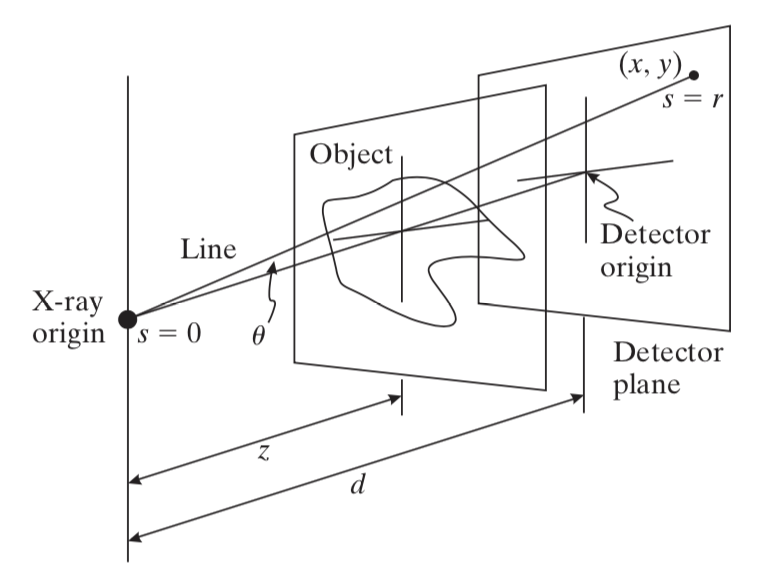
\includegraphics[width=8cm]{geometry_of_project.png}
    \caption{The geometry of a conventional projection radiographic system}
    \label{fig:geometry_of_project}%
\end{figure}

\paragraph{Question 3:} What determines the highest energy of X-ray photons emitted from an x- ray tube? What determines the energy spectrum of the X-ray photons?

\paragraph{Answer: } The peak value of X-ray tube voltage determines the highest energy of photons. For instance, the peak value of X-ray energy is $P$ $keV$ for the peak X-ray tube voltage is $P$ $kV$. 

The energy spectrum of photons is the sum of characteristic X-ray spectrum and bremsstrahlung X-ray spectrum. The characteristic X-ray energy being released depends on the energy difference between the outer and the inner shell in atoms at the X-ray tube's anode. The bremsstrahlung X-ray energy being released depends on how close the incident electron passes the nucleus in the X-ray tube's anode.  

\paragraph{Question 4:} Compare characteristic radiation and bremsstrahlung radiation. What are their similarities and differences?


\paragraph{Answer: } 
Differences: 
\begin{center}
    \begin{tabular}{ |p{8cm} | p{8cm} |}
    \hline
    Characteristic & Bremsstrahlung \\ \hline
    Characteristic radiations are generated by electrons lose their kinetic energy excitation and ionization & Bremsstrahlung radiations are generated through slowing down the electrons by passing the nucleus of an atom. \\ \hline
    Characteristic radiations are a collection of discrete energy level since the excess energy being released as X-rays depends on the energy difference between the outer and the inner shell & Bremsstrahlung radiations are continuous since the energy levels are continuous \\ \hline
    As atomic number increases, characteristic radiations increases & As kV increases, bremsstrahlung radiations increase \\ \hline
    Referred to as monochromatic radiation & Referred to as polychromatic radiation \\ \hline
    \end{tabular}
\end{center}

Similarities:
\begin{itemize}
    \item Electrons gain kinetic energy by heading the cathode and accelerated toward the anode. Both characteristic and bremsstrahlung radiations are generated due to electrons from the cathode lose kinetic energy at the anode. 
    \item The excess energy in both characteristic and bremsstrahlung radiations are emitted as photons.
\end{itemize}

\paragraph{Question 5: } Using relativistic equations, determine the speed of an electron that is accelerated across a 120 kV potential in the X-Ray tube.

\paragraph{Answer: } Assume $m_0$ is the rest mass of the electron, which is $9.10938 \times 10^{-31} kg$. We also know that:

\begin{equation}
    1eV = 1.60218 \times 10^{-19} J
\end{equation}
Therefore,
\begin{equation}
    1J = 6.242 \times 10^{18} eV
\end{equation}
We can derive $E_0$
\begin{equation} \label{eq1}
\begin{split}
E_0 & = m_0c^2 \\
& = 9.10938 \times 10^{-31} \times (3\times10^8)^2 \times 6.242 \times 10^{18}\\
& = 511 keV
\end{split}
\end{equation}

The kinetic energy of a particle is the difference in energy between the moving particle and the stationary particle:

\begin{equation} \label{eq1}
\begin{split}
KE & = mc^2 - m_0c^2 \\
& = \frac{m_0c^2}{\sqrt{1 - \frac{v^2}{c^2}}} - m_0c^2 \\
& = m_0c^2(\frac{1}{\sqrt{1 - \frac{v^2}{c^2}}} - 1)
\end{split}
\end{equation}
Since the electron is accelerated across a $120 kV$ potential in the X-Ray tube, we know that the kinetic energy of the electron is $EK = 120keV$

From (8), we derive the following:
\begin{equation}
\frac{KE}{m_0c^2} = \frac{1}{\sqrt{1 - \frac{v^2}{c^2}}} - 1
\end{equation}

\begin{equation}
\frac{120keV}{511keV} = \frac{1}{\sqrt{1 - \frac{v^2}{c^2}}} - 1
\end{equation}

\begin{equation}
\frac{120keV}{511keV} = \frac{1}{\sqrt{1 - \frac{v^2}{c^2}}} - 1
\end{equation}

After some simple algebra, we obtain:
\begin{equation}
v = 0.5867c
\end{equation}

Hence, he speed of an electron that is accelerated across a 120 kV potential in the X-Ray tube is $v = 0.5867c$, where $c$ is the speed of light.

\paragraph{Question 6}: If 80\% of X-ray photons of a certain energy pass through a slab of material, what percentage passes through a slab of the material which is twice as thick as the original slab?

\paragraph{Answer:}
The attenuation relationship of X-ray photons of a certain energy pass through a slab of material is given as:

\begin{equation}
I = I_0e^{-\mu t}
\end{equation}

where $\mu$ is the attenuation coefficient of the tissue and $t$ is the thickness of the tissue. 

From the Question, we know that

\begin{equation}  \label{eq1}
\begin{split}
    I & = I_0e^{-\mu t} \\
      & = 0.8I_0 \\
\end{split}
\end{equation}


Suppose $t' = 2t$, and take $\ln$ on both sides of $(14)$:


\begin{equation}  \label{eq1}
\begin{split}
    \ln I & = \ln I_0 - \mu t \\
          & = \ln I_0 + \ln0.8 \\
\end{split}
\end{equation}
Therefore, we know that $\ln0.8 = -\mu t$.

Suppose the $I'$ is the intensity of photons pass through a slab of material that is twice as thick as the original slab, and $t' = 2t$.

\begin{equation}
    I' = I_0e^{-2\mu t}
\end{equation}
Take $\ln$ on both sides of $(16)$

\begin{equation}  \label{eq1}
\begin{split}
    \ln I' & = \ln I_0 - 2\mu t \\
          & = \ln I_0 + 2\ln0.8 \\
          & = \ln I_0 + \ln0.64 \\
\end{split}
\end{equation}

And we take $e$ exponent on both sides of $(17)$:
\begin{equation}  \label{eq1}
\begin{split}
    I' & = I_0e^{-2\mu t} \\
       & = 0.64I_0 \\
\end{split}
\end{equation}

Hence, 64\% of $I$ pass through a slab of the material which is twice as thick as the original slab.

\paragraph{Question 7: }A chest radiograph is 36cm$\times$43cm. If we want to preserve all the detail in the image, to a spatial resolution $5mm^{-1}$, how many pixels would be required? What will be the size of the image, if quantization were performed on 256 gray levels?

\paragraph{Answer: } By Nyquist Shannon sampling theorem, we know if we want to retain all detail information, the image needs to be sampled at a sampling frequency, $f_s$, that is at least twice that of the highest frequency ($f_{max}$) contained in it;

\begin{equation}
    f_s \geqslant 2 \times f_{max}
\end{equation}

Therefore, since the spatial resolution of the image is $5mm^{-1}$, by Nyquist Shannon sampling theorem, we need to sample 10 pixels $mm^{-1}$, i.e., 10 pixels taken per millimeter. Therefore, each pixel is 0.1 milimeter. 

Since 1 $cm$ = 10 $mm$, we need 3600 $\times$ 4300 pixels, which equals 15,480,000 pixels. Each pixel has 8 bit (1 byte) to represengt 256 gray level, so we need 15,480,000 pixels $\times$ 1 byte = 15,480,000 bytes (15.48 Megabyte, or 15.48 MB) to store the image. 

\end{document}


%%% Local Variables:
%%% mode: latex
%%% TeX-master: t
%%% End:
